\documentclass{article}
\usepackage{graphicx}
\topmargin  0.0in
\headheight  0.15in
\headsep  0.15in
\footskip  0.2in
\textheight 8.45in

\oddsidemargin 0.56in
\evensidemargin \oddsidemargin
\textwidth 5.8in

%%\usepackage{clrscode}
%%\input{epsf}

\pagestyle{myheadings}
\markright{\bf Volume Grid Format}

\begin{document}

\title{The Volume Grid (vog) File Format}

\author{ Edward Luke \\
\it luke@cse.msstate.edu}


\maketitle

% example of figure including code
%\begin{figure}[htbp]
%  \centerline{ \epsfxsize=5.5in \epsfbox{figures/constructs.eps}}
% \caption{Four Basic Container Categories}
% \label{constructs}
%\end{figure}

\section{Introduction}

The volume grid file format is a format implemented using the HDF5
library.  The contents of the file include the following top level
groups: {\tt file\_info}, {\tt node\_info}, {\tt surface\_info}, and
{\tt face\_info}.

\subsection{\tt file\_info}

The {\tt file\_info} group contains general information about the mesh.  This
includes the following attributes:
\begin{enumerate}
  \item {\tt numCells} : integer describing the number of cells in the mesh.
  \item {\tt numFaces} : integer describing the number of faces in the mesh.
  \item {\tt numNodes} : integer describing the number of nodes in the mesh.
\end{enumerate}

\subsection{\tt node\_info}

The {node\_info} group contains an array of 3-D vectors in a dataset
under the name {\tt positions}.  This array has a length equal to the
{\tt numNodes} attribute given in the {\tt file\_info} group.


\subsection{\tt surface\_info}

The {\tt surface\_info} group contains boundary condition information.
For each named boundary condition this group contains a group with the
name of the boundary surface. Under this group is an attribute {\tt
  Ident} that contains the integer tag associated with this boundary.
This tag will be how the boundary faces are identified in the {\tt
  face\_info}

\subsection{\tt face\_info}.

The {\tt face\_info} group contains a compressed data structure that
identifies the nodes and cells associated with each face.  The
compression factor this data structure provides depends on the
locality of the data within the mesh.  Usually cells are ordered using
a space filling curve to improve compression as well as to help
improve performance of parallel file processing.  The node and face
orderings are also optimized to improve locality and increase
compression of these data structures.  In this data structure faces
are written out in small clusters of variable size.  The {\tt
  cluster\_sizes} data set is an array of the size in bytes of each
cluster, while the attribute {\tt cluster\_info} dataset is a
concatenation of all face clusters.

The face clusters store, in a compressed form, the nodes that form a
face and the cells that lie on the left and right sides of the face.
These relationships are identified as {\tt face2node} that lists the
nodes that form the face in an ordering that defines a normal vector
that points out of the left cell and into the right cell.  The cells
on either side of a face are defined by {\tt cl} (cell left) and {\tt
  cr} (cell right) according to the right hand rule as illustrated in
figure \ref{fig:face}.  Cells are numbered starting from $0$ while
negative cell numbers are reserved for marking boundary surface facets
with a surface identifier.  All boundary faces are oriented so that
the normal points out of the domain such that {\tt cr} right cell will
contain a negative of the boundary surface id associated with that
boundary face.  Finally for all interior faces (faces in which {\tt
  cl} and {\tt cr} are positive numbers) the face must be oriented
such that there exists some unique coloring that can be applied to the
cells where the left cell has a lower color than the right cell.  In
other words, the faces are oriented such that one cannot follow faces
from left to right and ever arrive back to the same cell from which
they started.  This coloring is used when the symmetric Gauss Seidel
solver is employed and is usually determined by the level parameter
that is obtained from a depth first search of cell-to-cell
connectivity implied by the faces.

\begin{figure}[htbp]
\begin{center}
  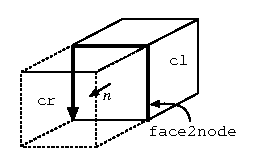
\includegraphics[width=10cm]{face}
 \caption{The {\tt face2node} map and its relationship to neighboring cells}
 \label{fig:face}
\end{center}
\end{figure}

\subsection{Optimizing Mesh Element Ordering}

Face clusters are designed to compactly store face connectivity
information in a compressed form that can dynamically expand to an
arbitrary number of bits for identifiers.  The compression as well as
parallel reading efficiency of the file can be improved if the mesh
elements are renumbered to increase locality.  These optimization
are not required but tend to reduce file size and improve solver
performance.  The current optimization scheme uses space filling
curves (Hilbert Curve) to enhance spatial locality.  The optimization
follows the following steps starting with the un-optimized mesh:

\begin{enumerate}
  \item Compute cell centers
  \item Determine Hilbert key, Reorder (sort cells) according to
    Hilbert space filling curve
  \item Reorder faces according to first visited order when passing
    through cells in optimized order
  \item Reorder nodes according to first visited order when passing through
    faces in optimized order.
\end{enumerate}

The resulting mesh will allow more faces to be packed into each face
cluster but will also improve cache performance when processing the
mesh by the Loci file reader and subsequent solver steps.

\subsection{Matrix Coloring}

The matrix coloring phase determines the left-right assignment of
faces in the mesh.  The left-right ordering must correspond to a
coloring for some of the linear system solvers to function correctly.
Some matrix coloring will give better linear system solver
performance.  A good coloring can be defined by coloring according to
the order that a depth first search of the cell-to-cell connectivity.
When running in parallel, use the space-filling curve described above
to partition the mesh and perform the depth first search within each
processor.

\subsection{Face Cluster Data Structure}

The face cluster stores connectivity information using unsigned
char data and then includes a translation table to convert these
unsigned char representations to an arbitrary precision integer
format.  Therefore a cluster can refer to at most 256 distinct nodes
and 256 distinct cells.  The number of faces that can be packed into a
clusters is determined by iterating over faces until either the number
of unique nodes or cells accessed exceeds 256.  The faces are then
encoded using the following encoding protocol:
\begin{enumerate}
  \item First the number of nodes in the face is provided (A zero
    means this is the end of the face information in the cluster)
    followed by the number of faces of this size.
  \item For each face of that size the nodes are listed and then the
    left and right cell. (Boundary faces will have a negative number in
    the right cell which is the boundary facet id.)
  \item If the number of faces of the same side happens to exceed 255,
    then the remaining faces will be encoded in the next face block.
  \item If the number of nodes in the face is zero, then there will be
    no more face information and the translation tables will follow.
\end{enumerate}

The protocol described above is illustrated in figure
\ref{fig:clusterencoding} where {\tt fsz} is the number of nodes that
describe the face (e.g. 3 for triangle, 4 for quad), {\tt nfc} is the
number of faces of that size, {\tt nd}{\em x} is are the nodes that
form the face, and {\tt cl} and {\tt cr} are the left and right cells.


\begin{figure}[htbp]
\begin{center}
  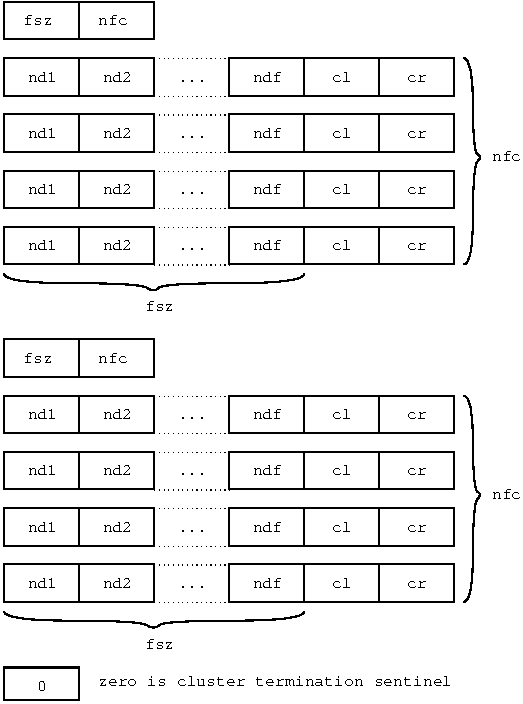
\includegraphics[width=10cm]{fcluster}
 \caption{The face encoding within a face cluster.  Each block is a byte.}
 \label{fig:clusterencoding}
\end{center}
\end{figure}


Then next part of the face cluster are the maps that list the global
node and cell ids that translate from the cluster local numbering
(using bytes) to the global file numbering.  The node table is written
first followed by the cell table.  The first entry in the table is the
number of items in the table followed by a list of arbitrary precision
formatted integers with one for each table entry.  The most
significant bit of every byte is the continue bit, if it is set then
the number continues to the next byte.  For the first byte in the
number the bit defined by {\tt 0x40} is the sign bit which is set if the
number is negative.  The next 6 bits is the Least Significant Bits of
the number.  Each subsequent byte adds 7 more bits to the integer in 
increasing significance.  The end of the integer is indicated by a byte
that has a zero in MSB defined by {\tt 0x80}.   This format allows the
mesh format to represent identifiers up to 64 bits without uniformly
adding a 64 bit storage cost.


\end{document}
